\chapter{Characterization \& Benchmarks}

  The matrix-vector multiplication performance of the C3SR format is measured in its CSR-like and vectorized implementations (see \ref{subsec:matrix-vector-multiplication-schemes}). Firstly, a baseline performance is established by comparing the matrix-vector multiplication performance of the C3SR format's CSR-like multiplication scheme introduced in \ref{subsubsec:basic-csr-like-multiplication-scheme} against the CSR format's performance on different sparse banded matrices derived from structured grids and on three different machines. Secondly, the C3SR format's baseline performance is compared against its vectorized counterpart introduced in \ref{subsubsec:vectorized-simd-multiplication-scheme}.

  The following subsection introduces the sparse banded matrices used for the performance benchmarks and their method of acquisition. Subsequently, the results of the performance benchmarks are discussed. Information on the machines used for the benchmarks can be found at the ASC infrastructure wiki\footnote{https://mp-force.ziti.uni-heidelberg.de/kmbeutel/personal-wiki/wikis/ASC-infrastructure} (the KNL was configured to 50\% hybrid mode). All benchmarks were run multi-threaded utilizing the machines' full hardware capabilities.

  \section{Generation of Sparse Banded Matrices as Test Matrices}

    For the purpose of gauging the arithmetic performance, test matrices are created. These matrices resemble the structure of the sparse banded matrices introduced above and are created by iterating through a 3D grid of fixed integral dimensions X, Y, Z and applying a given stencil operation which encodes the desired adjacency relationship of the grid. Nodes requested by the stencil but missing from the grid, i.e. nodes on the grid's outer borders, are omitted, i.e. their corresponding entries in the adjacency matrix carry a zero corresponding to Dirichlet-type boundary conditions.

    The matrix's non-zero entries' numeric values are obtained from evaluating a sinusoidal function at the geometric center point $\vec{r} = (x, y, z)$ inbetween the two nodes in question whereby each Cartesian component $x, y, z$ is scaled by its coordinate's span $X, Y, Z$. An additional offset serves to prevent that entries in the matrix correponding to adjacent nodes according to the stencil incidentally evaluate to 0. The function utilized is $$W(x,y,z; n_x, n_y, n_z) = 2 + \sum \limits_{d \in \{x,y,z\}} \sin{\frac{d}{d_{\text{max}}} \cdot \pi \cdot n_d} $$ where $n_x, n_y, n_z$ are periodicity parameters for each dimensions. The matrix in Figure \ref{fig:laplacian-example} has been created using this method.

    Note that $n_d = 0 \Leftrightarrow \partial_d W(\vec{r}) \equiv 0$, introducing a periodicity in the corresponding dimension $d$. This feature is utilized to control the periodicity in the matrix's values.

    For the purpose of this work two different sets of parameters are utilized generating two different matrices: A smaller matrix generated from a $100 \times 100 \times 100$ grid with the periodicities $n_x = n_y = n_z = 0$ and a second matrix based on the same grid but different periodicities $n_x = 1.1; n_y = 1.2; n_z = 1.3$. Both matrices are generated from a symmetric 7p-stencil operation. The matrices' structures are their grid's equivalent to the example shown in Figure \ref{fig:laplacian-example}.

    The first matrix's values are identical for all rows whose pattern is the same such that \V and \J contain the same small number of elements. The second matrix's rows' values are all unique and thus \V contains approximately $7 \cdot 100^3$ elements (Figure \ref{fig:matrix_stats}).

    \begin{figure}[ht]
      \centering
      \begin{tabular}{ l | c c }
          Array & First Matrix & Second Matrix       \\
        \hline                                       \\
        \V         & $135$          & $6940000$      \\
        \VS        & $1000000$      & $1000000$      \\
        \J         & $135$          & $135$          \\
        \JS        & $1000000$      & $1000000$      \\
        \JP        & $1000000$      & $1000000$      \\
        \RS        & $1000000$      & $1000000$      \\
        Total Size in C3SR format & $\approx 16$MB & $\approx 72$MB \\
        Total Size in CSR Format & $\approx 87$MB & $\approx 87$MB \\
        \hfill
      \end{tabular}
      \caption[Matrices in C3SR format used for matrix-vector multiplication benchmarking.]{\textbf{Matrices in C3SR format used for matrix-vector multiplication benchmarking.} Number of elements is displayed for each array. \V stores double-precision floating-points while all other arrays use 32 bit-wide integers. Additionally, the matrix's size in CSR representation is listed.}
      \label{fig:matrix_stats}
    \end{figure}

    Note that the two matrices share the same structure and thus their only difference is found in \V and \VS. Concerning the vectorized matrix-vector multiplication scheme the first matrix primarily utilizes scheme II (Figure \ref{fig:simd_scheme_diag_collated}) while the second matrix mainly relies on scheme I (Figure \ref{fig:simd_scheme_diag}). The matrices are generated using the asc::matrixgen C++ library\footnote{https://mp-force.ziti.uni-heidelberg.de/asc/AscMatrixGen}.

  \section{Performance of CSR-like Matrix-Vector Multiplication}

    The C3SR format's CSR-like matrix-vector multiplication scheme (referred to as \emph{baseline implementation} hereinafter; see \ref{subsubsec:basic-csr-like-multiplication-scheme}) is compared against its CSR format's pendant using the Eigen C++ library \cite{eigen:website} on three different machines using the sparse banded matrices introduced in the previous section. The results are displayed in Figure \ref{fig:baseline_arithmetic_performance}.

    \begin{figure}[!ht]
      \centering
      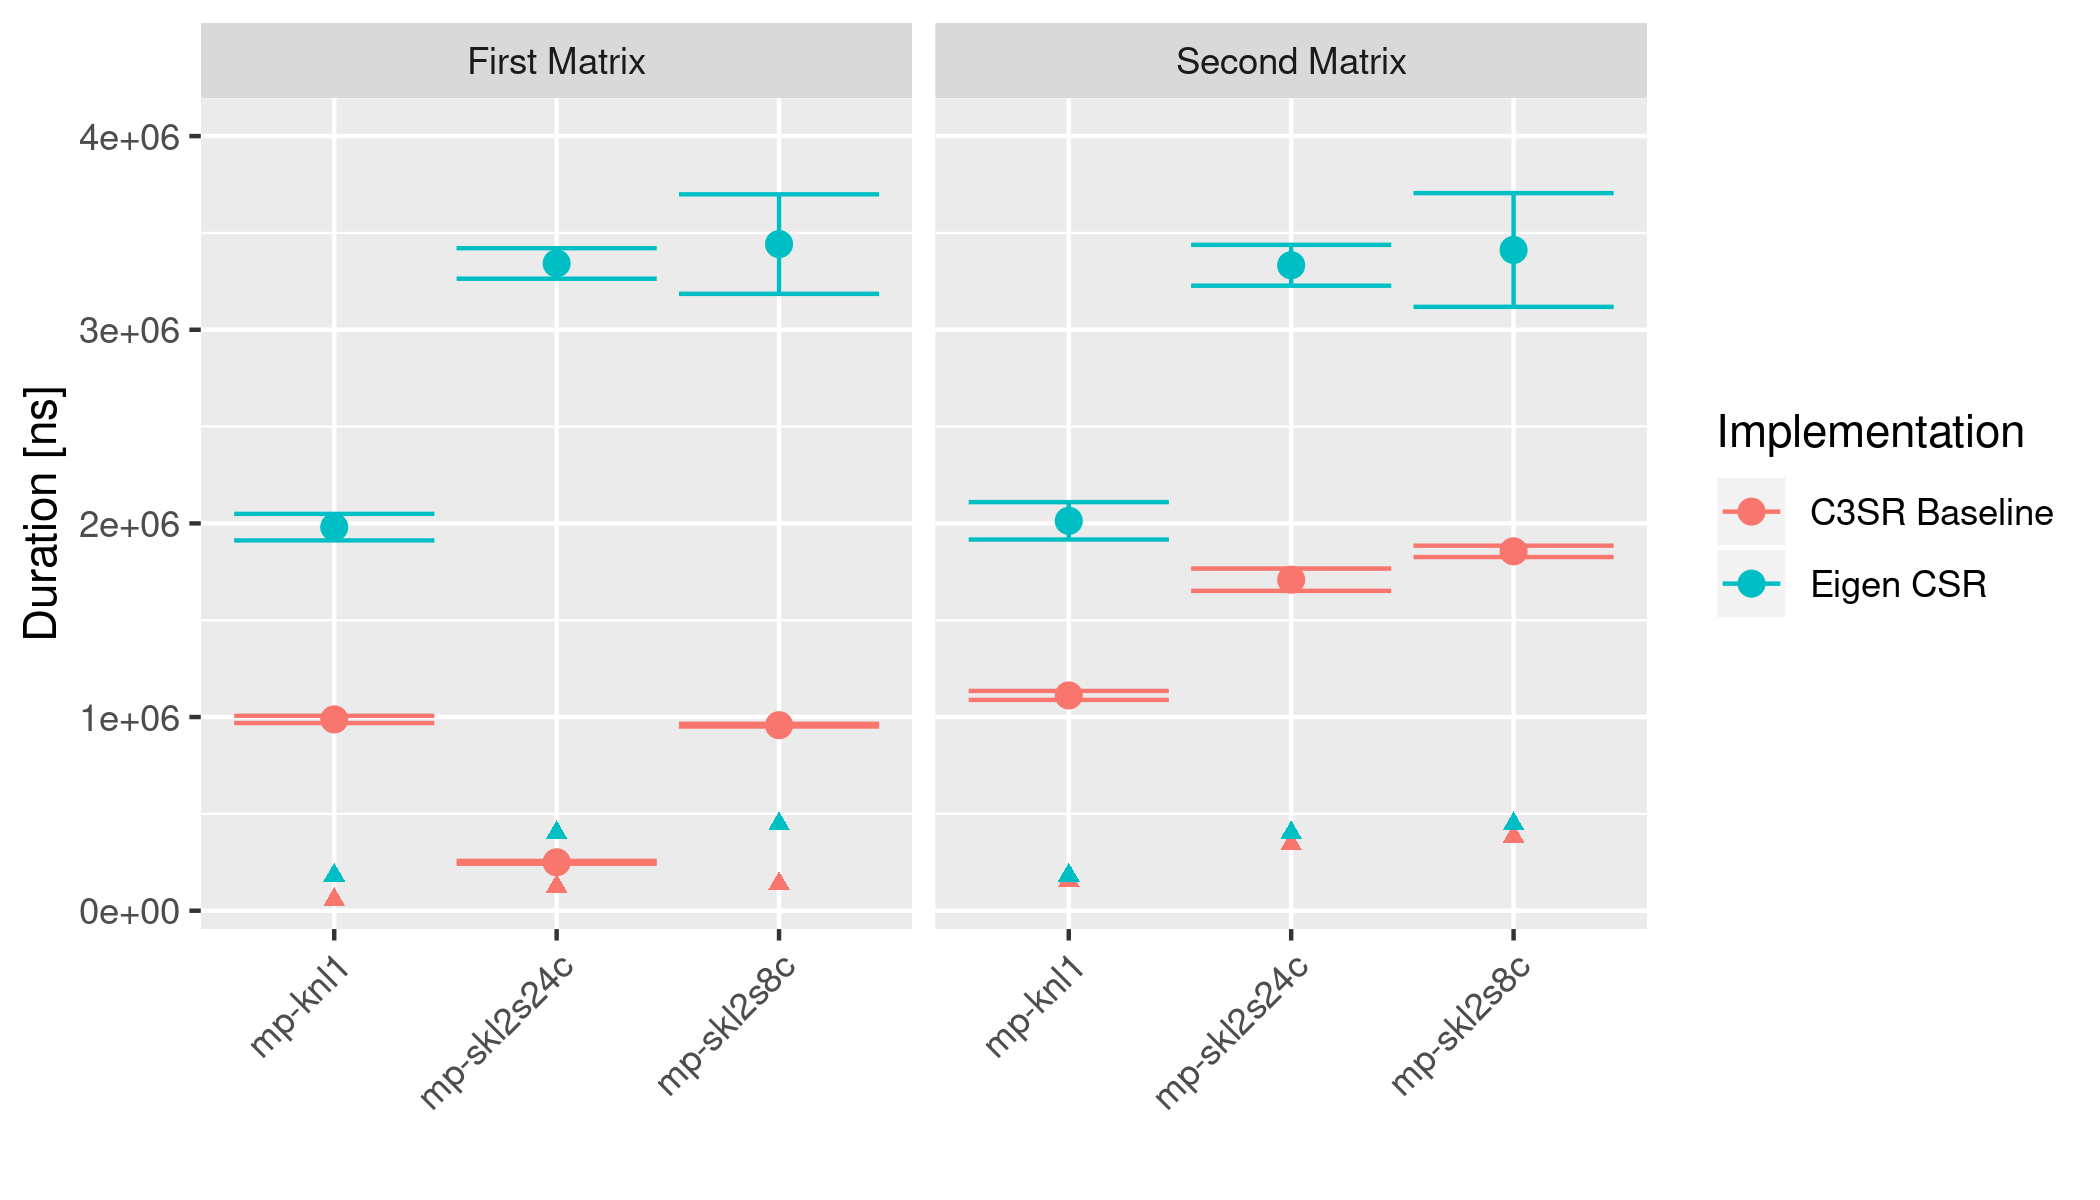
\includegraphics[width=0.9\textwidth]{assets/eigen_vs_c3sr_baseline}
      \caption[Performance comparison of the CSR format against the C3SR format on sparse banded matrices.]{\textbf{Performance comparison of the CSR format against the C3SR format on sparse banded matrices.} The means and sample standard deviations of $10$ samples à $10000$ consecutive matrix-vector multiplications are shown. As the CSR format's representation of the different matrices is identical except for differing numeric values the arithmetic performance is the same save for statistical variance. The triangular symbols denote the theoretical limits as determined by the quotient of the total amount of data involved in a matrix-vector multiplication and the system's theoretical memory bandwidth. Since the matrix storage sizes differ between the storage formats two different limits are displayed.}
      \label{fig:baseline_arithmetic_performance}
    \end{figure}

    By design of the C3SR format, it outperforms the CSR format in the order of magnitude of around $50\%$ irrespective of the machine. This is due to the reduction in the size of the representation of the matrices and the consequent improvement in data locality as the C3SR format's arithmetic is slightly more complex as discussed in \ref{subsubsec:basic-csr-like-multiplication-scheme}. Accordingly, the performance improvement is more pronounced for the first matrix, whose storage size is smaller, entailing speed-up factors of approximately 2, 13, and 3.

    Despite the clear performance benefits the above results have to be qualified further as the implementation of the C3SR format\footnote{https://mp-force.ziti.uni-heidelberg.de/shuell/c3srmatrix} uses a NUMA-aware memory allocation scheme for its data arrays, correctly distributing them across physical memory, suitable for the multi-socket systems utilized for the benchmarks. Conversely, the Eigen C++ library, a general purpose linear algebra and numerics framework, does not tailor its data fields' memory layout in such a way that might lead to performance penalties due to a data distribution inadequate for the access patterns of the multi-threaded arithmetic. Additionally, Eigen internally uses the multi-threading framework OpenMP \cite{openmp:website} which entails a dynamic overhead not present in the implementation of the C3SR format.

  \section{Performance of SIMD Matrix-Vector Multiplication}

    The C3SR format's vectorized multiplication scheme's performance is measured by comparing it against the baseline performance. The implementation of the vectorized multiplication scheme utilizes the explicit SIMD vectorization library UME::SIMD \cite{umesimd2017}. The results are displayed in Figure \ref{fig:arithmetic-performance}.

    \begin{figure}[!ht]
      \centering
      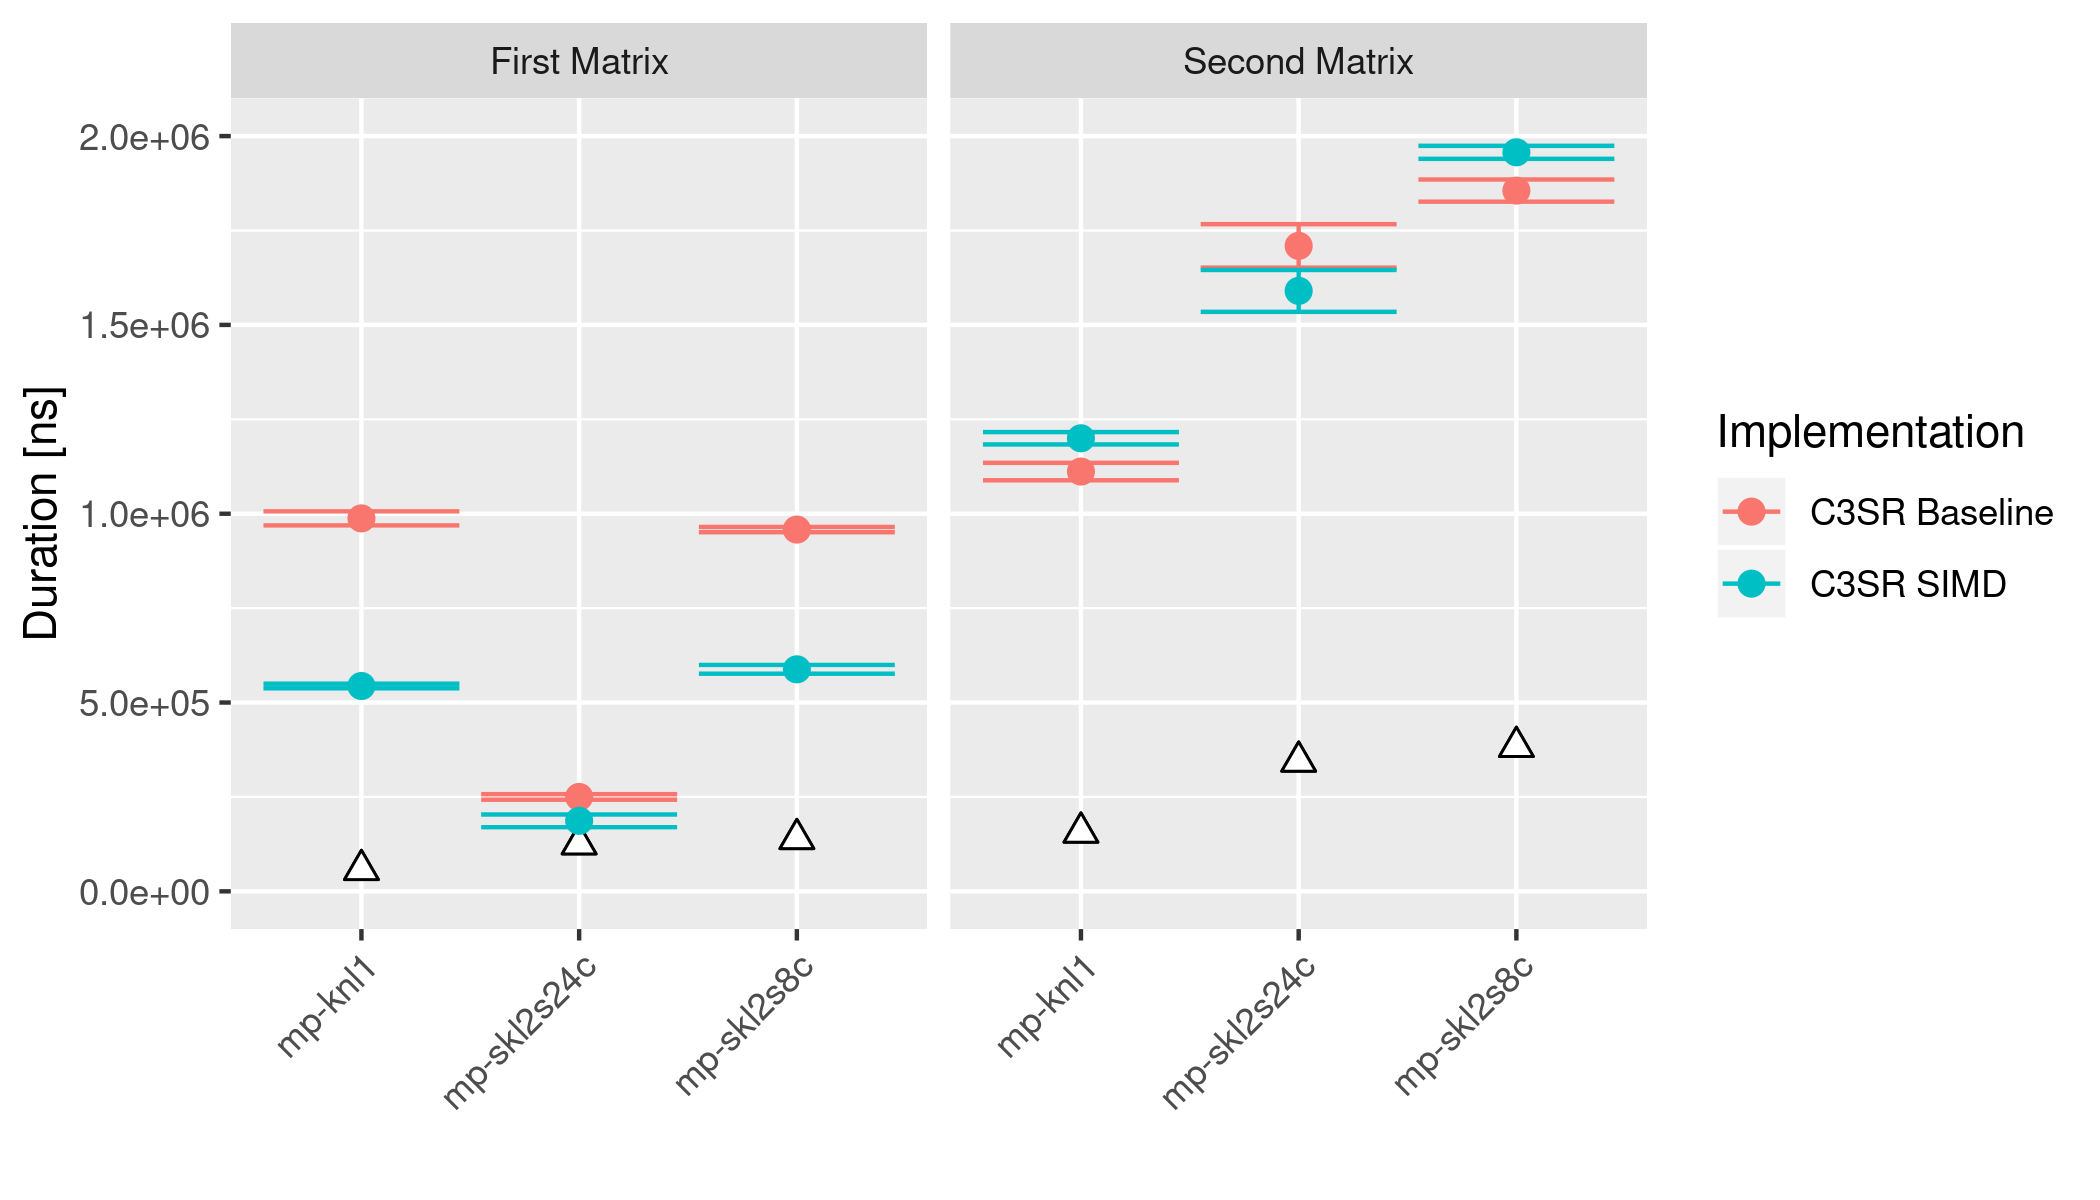
\includegraphics[width=0.9\textwidth]{assets/arithmetic_performance}
      \caption[Performance of C3SR vectorized matrix-vector multiplication scheme compared to baseline implementation.]{\textbf{Performance of C3SR vectorized matrix-vector multiplication scheme compared to baseline implementation.} The means and sample standard deviations of $10$ samples à $10000$ consecutive matrix-vector multiplications are shown. The triangular symbols denote the theoretical limits as determined by the quotient of the total amount of data involved in a matrix-vector multiplication and the system's theoretical memory bandwidth.}
      \label{fig:arithmetic-performance}
    \end{figure}

    Sparse matrix-vector multiplication is a memory-bound computation so that the efficacy of a vectorized arithmetic implementation depends very strongly on the amount of data that is required to be read from memory and whether the dynamic overhead involved in determining the applicable SIMD scheme is compensated by a speed-up in arithmetic. This fact is reflected in the measurements as for the second matrix the SIMD implementation is generally slower than the baseline implementation. Only for the first matrix a significant speed-up can be observed on every machine. However, this might be partly due to the fact that the second matrix's SIMD multiplication scheme is less performant as it involves strided loads from memory which might equate to regular gather operations on the hardware used for this benchmark (see \ref{subsubsec:vectorized-simd-multiplication-scheme}).

  \section{Further Considerations}

    By evidence of the performance benchmarks presented in the previous section the basis for the performance gain in the arithmetic of the C3SR format with respect to the CSR format for sparse banded matrices is the reduction of the matrix's total storage size in memory leading to big improvements in data locality during matrix-vector multiplication.

    The C3SR format's storage scheme is tailored to minimize the matrix' storage size in memory. However, depending on how the matrix object is created in memory, adhering to the storage scheme to its full extent may not be optimal as it might limit parallelism during object construction. The data arrays' contents are strongly coupled such that the workload cannot be trivially spread across multiple threads. Instead, it might be advisable to partition the matrix into equally sized slices whose independent C3SR objects can be created in parallel. Finally, these distinct C3SR objects corresponding to the matrix slices are then transformed into a singular object by concatenating the data arrays requiring that the index-pointer arrays are offset by the number of rows preceding their first matrix row.

    \begin{figure}[ht]
      \centering
      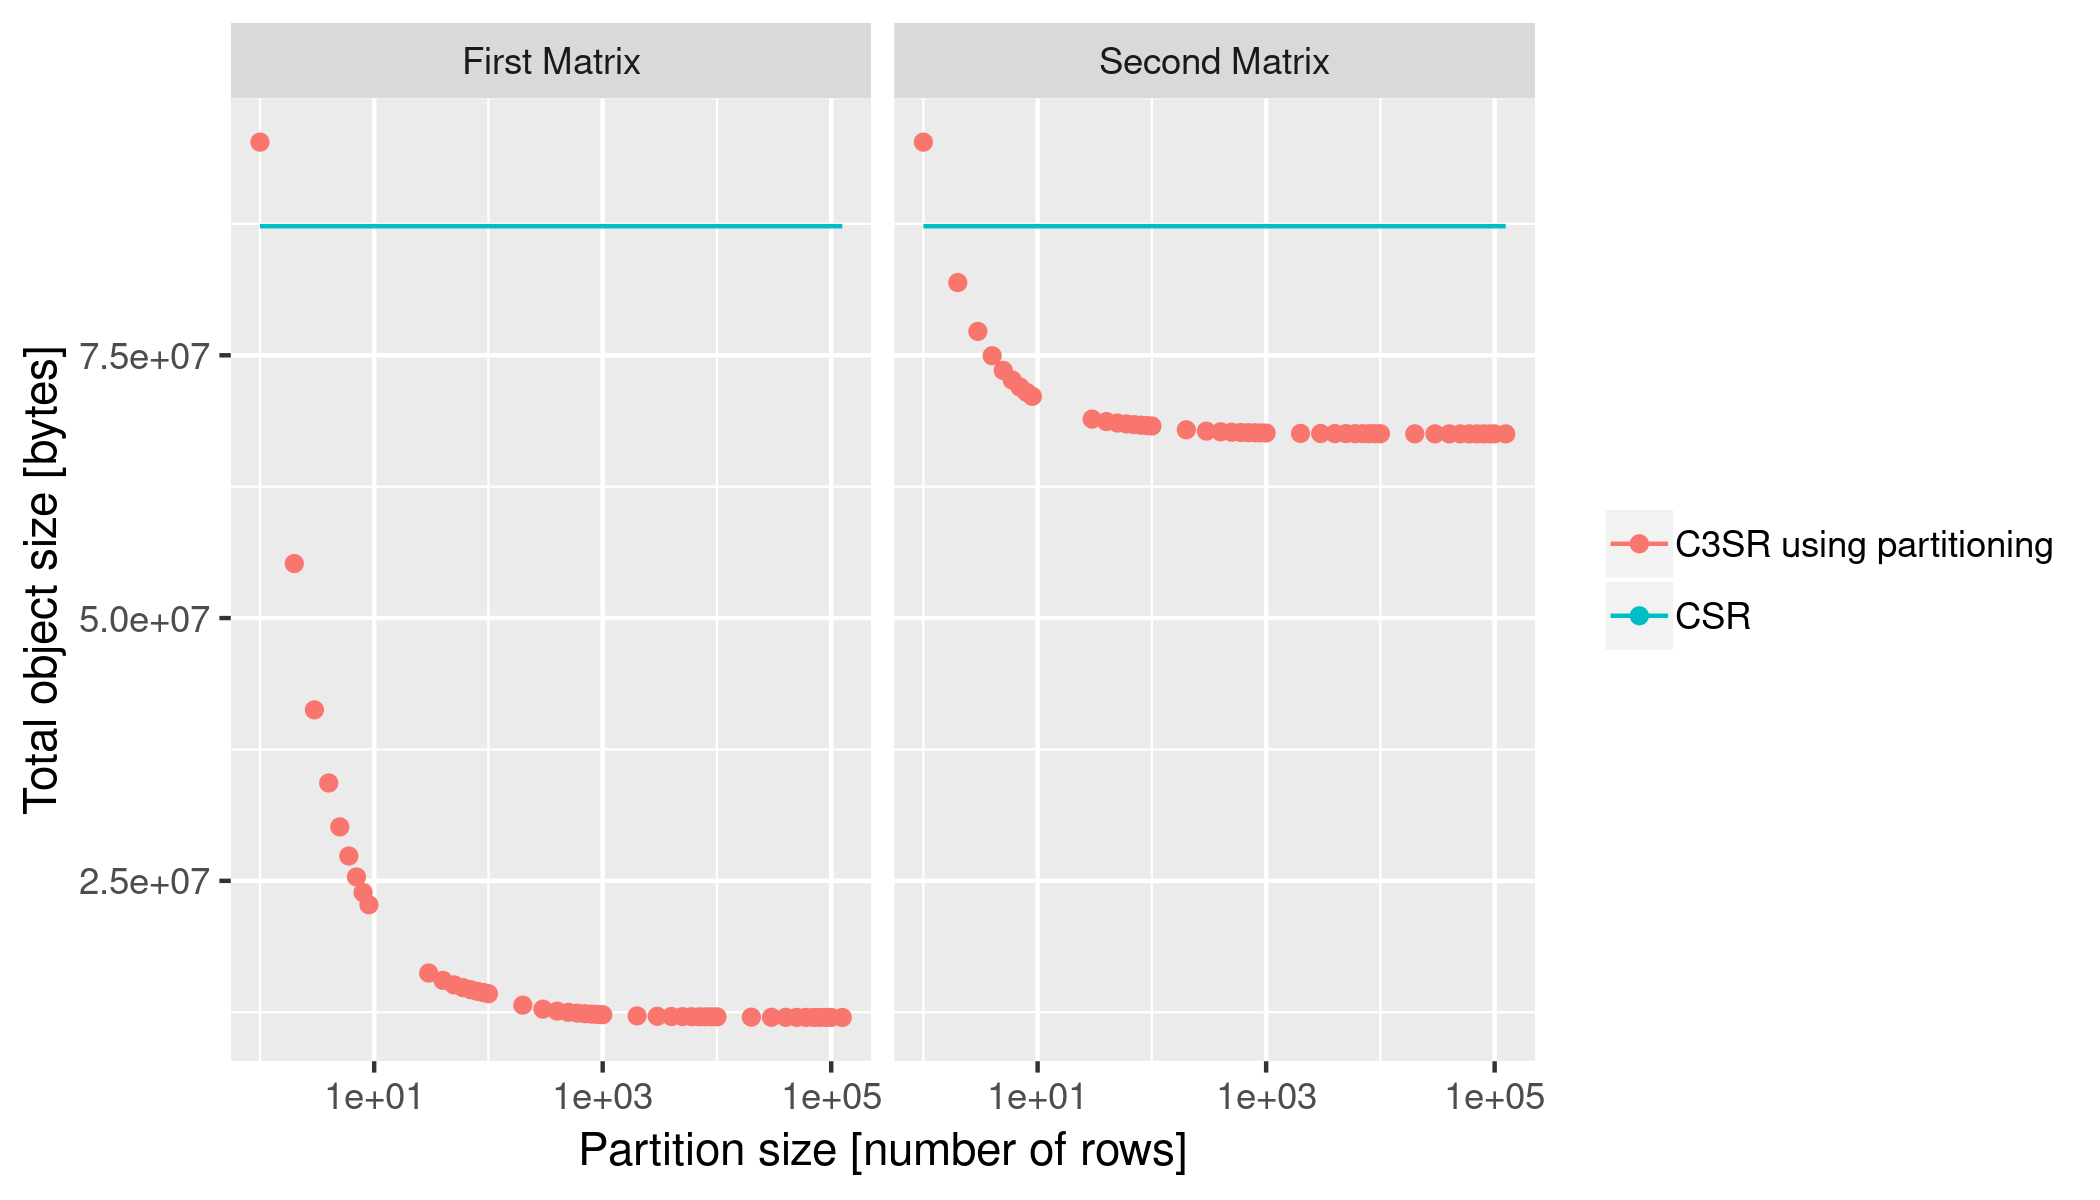
\includegraphics[width=0.9\textwidth]{assets/structured_grid_matrix_heap_size}
      \caption[C3SR matrix storage size depending on partition size.]{\textbf{C3SR matrix storage size depending on partition size.} Numeric values are stored using double precision floating-point numbers while all other arrays utilize 32 bit integers. A point of diminishing returns is reached at a partition size of around 1000, past which the storage size in memory does not shrink significantly. Thus, creating C3SR objects using partition sizes of 1000 and larger may yield a similar performance while speeding up the creation of the object. For comparison the corresponding CSR format's storage size is provided.}
      \label{fig:structured_grid_matrix_heap_size}
    \end{figure}

    In order to establish an estimate for an apt partition size Figure \ref{fig:structured_grid_matrix_heap_size} displays the total storage size depending on the partition size for the two matrices used for the performance benchmarks. It is evident that there exists a point of diminishing returns past whose partition size there is no significant gain in storage size reduction. This point is reached when the sizes of \V and \J, the two arrays responsible for the reduction in storage size for the C3SR format, fall significantly below the fixed sizes of the remaining arrays, which constitute a minimum to the storage size.

    Thus, the performance benefits of the C3SR format may be kept even when trading larger storage sizes in favor of the parallelizability of the application.

